% 软件  软件分析
%作者:赵启
%上次更新:2020年1月10日 17:20


\chapter{软件分析}

\section{综述}

  {\songti 在整个项目的设计与之后的装配分析中,我们均学习探索并使用了一些软件进行辅助性分析,
 这对于我们进行相关的材料选择、整体设计、寿命分析以及装配的整体合理性都有了很大的帮助。}

\section{基于Matlab分析的骨架设计}

  {\songti 在最开始的设计中,我们需要初步探索出最合适的大致臂长,以满足我们对于三个臂长
  的设计需求。对此,我们采用了数学软件Matlab进行了建模分析。}

  {\songti 首先,我们通过实地探访肯德基的各种产品,通过食品称、直尺获得了我们所需要
  夹取的食品的长、宽、高、内径、外径以及重量等参数。在各个数据中我们选取了最大重量的
  食物——可乐,作为我们的目标载荷。}

  {\begin{table}
    \centering
    \caption{KFC食物实地调研结果}
    \begin{tabular}{|l|l|l|l|l|}
    \hline
    
    食物 & 重量(g) & 长(cm) & 宽(cm) & 高(cm) \\ \hline
    黄金鸡块 & 100.5 & 12 & 7.2 & 4.2 \\ \hline
    薯条 & 80.5 & 5 & 4.5 & 5.1 \\ \hline
    鸡腿堡 & 202.5 & 11 & 11 & 6.8 \\ \hline
    蛋挞 & 60 & 6.5 & 3.8 & 2.8 \\ \hline
    可乐 & 460 & 8.8 & 6 & 13 \\ \hline
    
  \end{tabular}
  \end{table} }

  {\songti 对于三杆机械臂,我们进行了如图所示的建模,如图~\ref{fig:matlab建模} 所示。
  我们分别对基座和连杆的铰链和各个壁进行了分别编号和建系,并在末端加载可乐的重量作为
  负载,以及加入初步估计的连杆的重量以及电机的重量,连杆的重量由设计的体积、45号钢的密度
  由公式}

  \begin{equation}
    G= \rho Alg
  \end{equation}

  \begin{equation}
    \Sigma M=\Sigma Fl
  \end{equation}
  
  {\songti 可以计算出每个铰链所受弯矩的大小。}



  {\songti 之后,便可以在Matlab软件中对此三杆机构进行模拟建模,并输出Gif动图实时显示
  出在杆移动的过程中A、B、C三点的扭矩,如图~\ref{fig:Matlab输出扭矩} 所示。之后再在
  合理的结构条件下对三个杆的长度进行不断调整组合,从而得到在保证满足夹取条件的前提下(
  如图~\ref{fig:Matlab输出扭矩} 所示)获得尽可能地获取扭矩小的三杆长度组合。}

  {\songti 最终我们通过不断实验初步确定,通过Matlab计算得到当三杆长度分别为45cm、40cm
  、10cm的时候可以在最大移动范围(基座360°旋转的情况下)140cm左右承受扭矩的最大值为45$N\cdot{m}$ 。

  \begin{figure}[!htp]
    \centering
    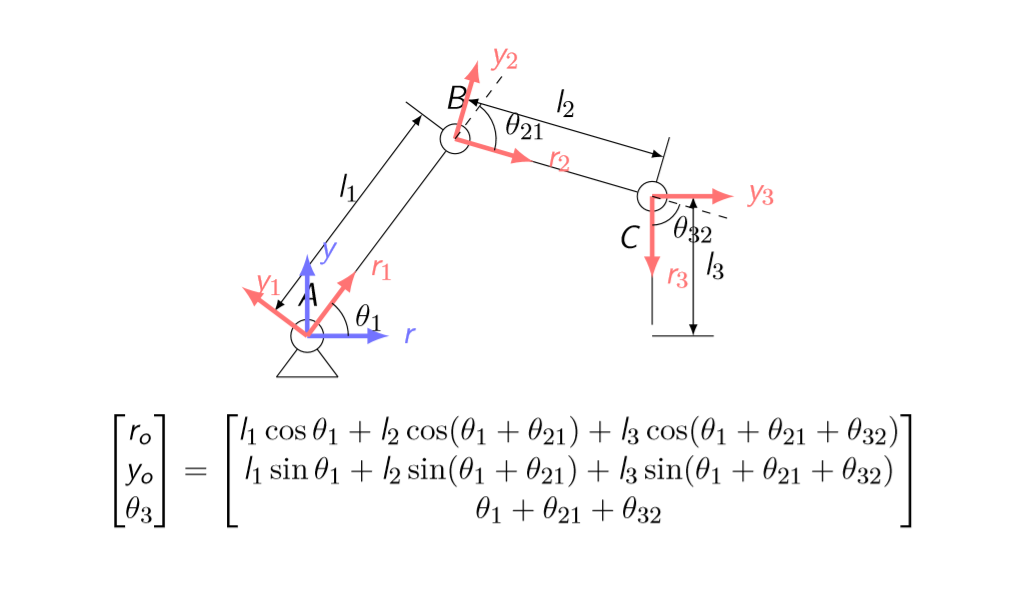
\includegraphics[width=15cm]{matlab_modeling.png}
    \bicaption[matlab建模]{matlab建模}{Matlab modeling}
    \label{fig:matlab建模}
  \end{figure}

  \begin{figure}[!htp]
    \centering
    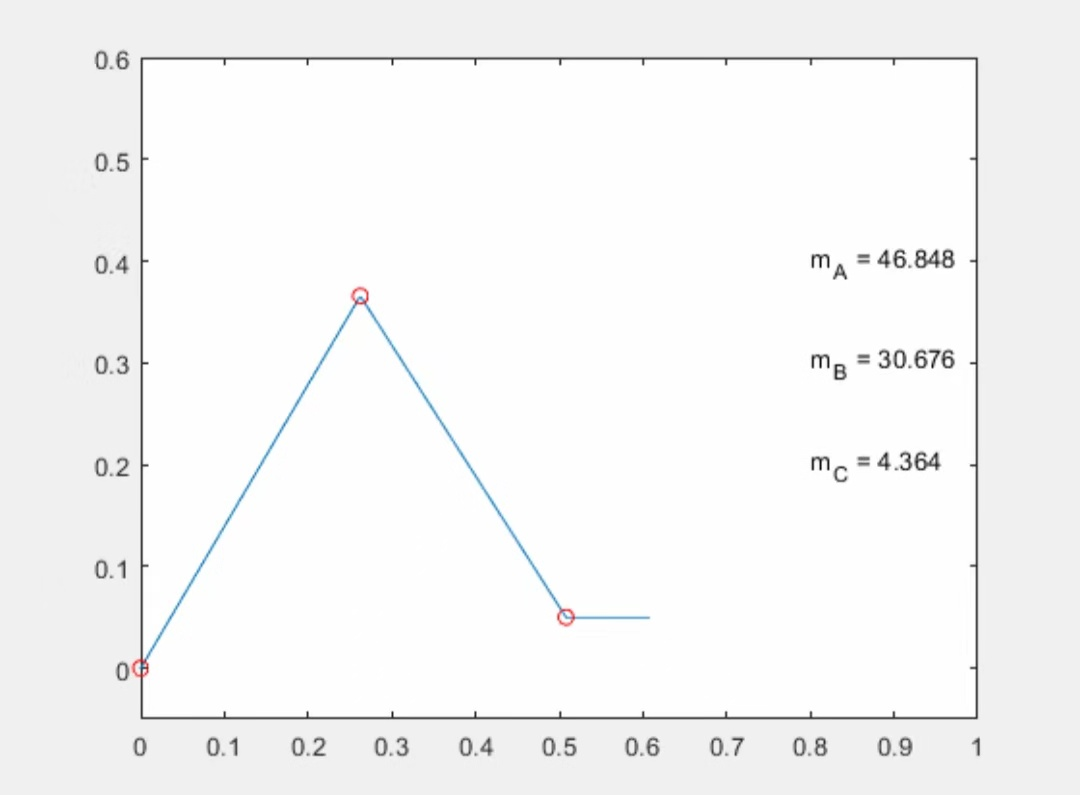
\includegraphics[width=12cm]{matlab_output_torque.jpg}
    \bicaption[Matlab输出扭矩]{Matlab输出扭矩}{Matlab torque outputing}
    \label{fig:Matlab输出扭矩}
  \end{figure}

  \begin{figure}[!htp]
    \centering
    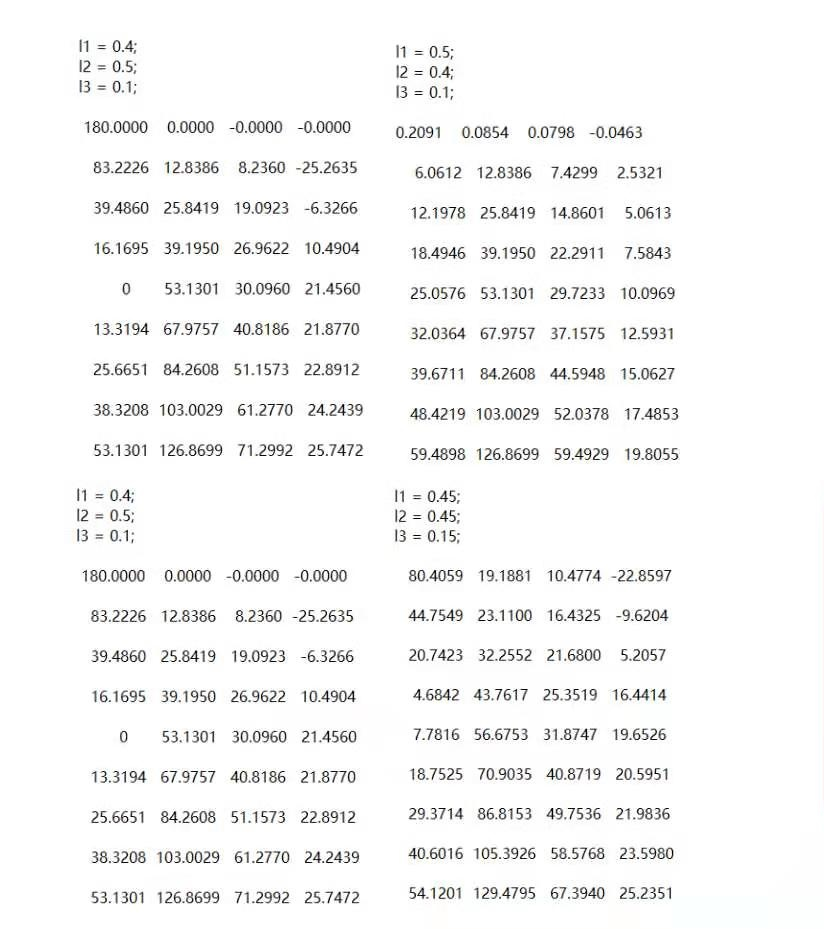
\includegraphics[width=12cm]{analysis_of_three-par_combinations_of_different_lengths.jpg}
    \bicaption[不同长度三杆组合分析]{不同长度三杆组合分析}{Analysis of three bar combination with different length}
    \label{fig:不同长度三杆组合分析}
  \end{figure}


\section{基于Ansys分析的蜗杆装配}

  {\songti 在实体装配的过程中,我们通过定性分析可知,基座上的蜗杆
  处于较下方的位置且其上装配有最多的轴承支座并和涡轮相啮合,
  因此会承受很大的应力并产生切变。出于对装配体的
  寿命和安全性的考虑,为了探究其切应力和正应力是否超过其屈服强度和切应力的许用值,我们
  利用Ansys进行有限元辅助分析。}
  
  {\songti 在Ansys中,我们根据装配体的结构情况,进行前处理、输入蜗杆的几何模型、对几何
  模型划分网格、根据装配体的实际情况施加载荷(图~\ref{fig:蜗杆的应力与扭矩}),求解后进行输出应力应变云图。}

  {\songti 在一开始我们设计的装配体中,蜗杆中央受到了极大的正应力,中间一部分超过了45号钢的屈服强度,因此极大地影响
  了蜗杆的工作和使用寿命(图~\ref{fig:改进前正应力})。之后,我们对上方装配体进行了一系列改进优化,如机械手部分尽可能
  采用3D打印结构并对其结构进行优化,并增加了支座分担蜗杆的应力,最终获得了较为理想的输出
  结果(图~\ref{fig:正应力})(图~\ref{fig:切应力})(图~\ref{fig:拉伸位移})} 。
   
  {\songti 由云图可以看出,改进后正应力极大降低,切应力也满足45号钢的许用值(除了极其微小的一部分稍微超过之外),能够满足蜗杆的安全工作条件。}
 
   

  \begin{figure}[!htp]
    \centering
    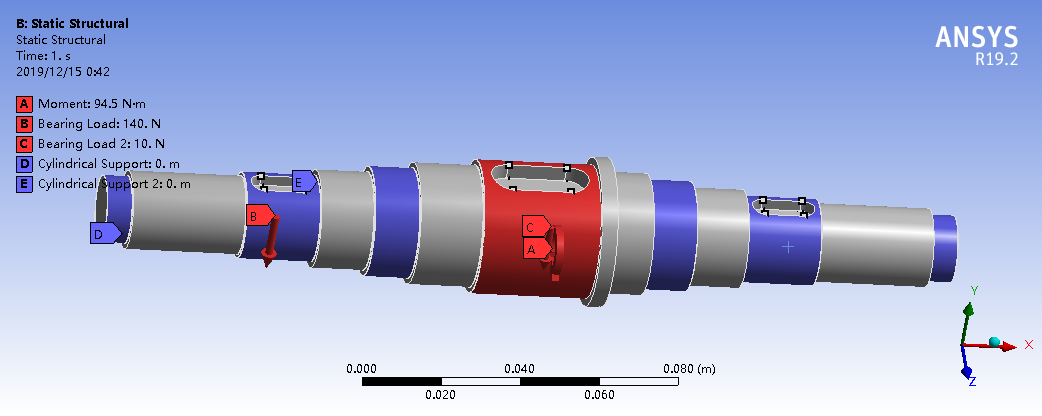
\includegraphics[width=12cm]{stress_and_torque_of_worm.png}
    \bicaption[软件蜗杆的应力与扭矩]{蜗杆的应力与扭矩}{Stress and torque of worm}
    \label{fig:蜗杆的应力与扭矩}
  \end{figure}

  
  \begin{figure}[!htp]
    \centering
    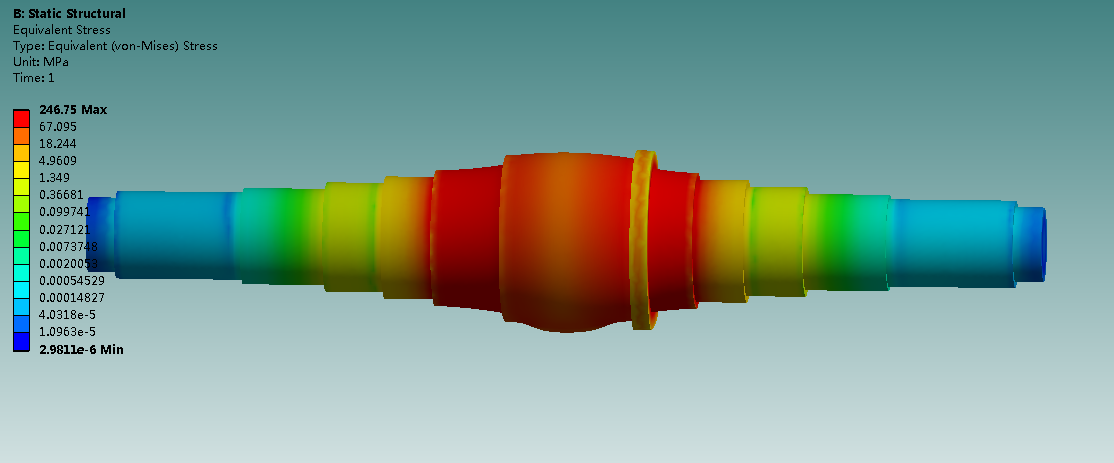
\includegraphics[width=12cm]{normal_stress_before_improvement.png}
    \bicaption[改进前正应力]{改进前正应力}{Normal stress before improvement}
    \label{fig:改进前正应力}
  \end{figure}

  
  \begin{figure}[!htp]
    \centering
    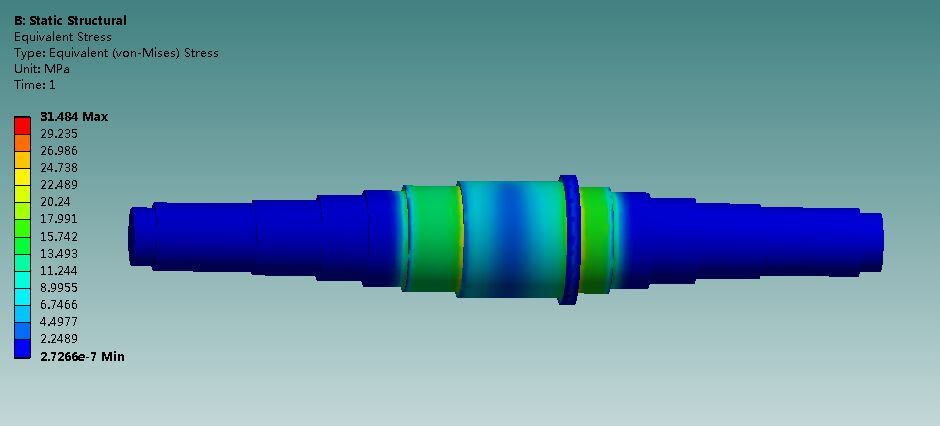
\includegraphics[width=12cm]{normal_stress.jpg}
    \bicaption[正应力]{正应力}{Normal stress}
    \label{fig:正应力}
  \end{figure}

  \begin{figure}[!htp]
    \centering
    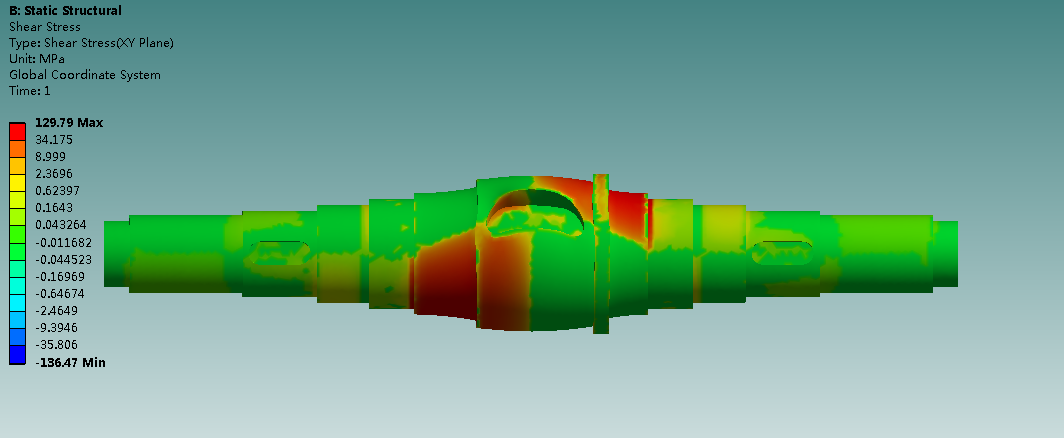
\includegraphics[width=12cm]{shear_stress.png}
    \bicaption[切应力]{切应力}{Shear stress}
    \label{fig:切应力}
  \end{figure}

  \begin{figure}[!htp]
    \centering
    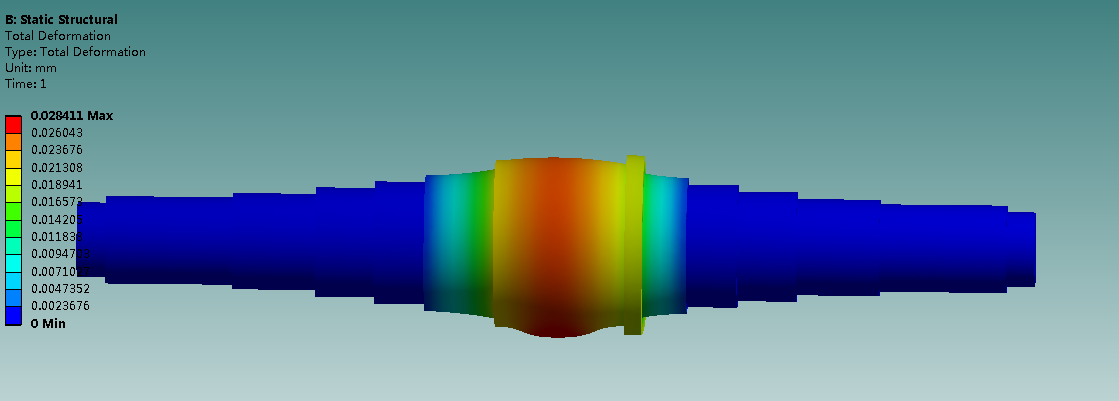
\includegraphics[width=12cm]{tensile_displacement.png}
    \bicaption[拉伸位移]{拉伸位移}{Tensile displacement}
    \label{fig:拉伸位移}
  \end{figure}

  \newpage

\section{基于ROS环境的机械臂分析}

{\songti 为了更好地去分析整个装置,我们小组尝试了Robot Operating System机器人操控系统(以下简称ROS),首先,我们下载安装了了Ubuntu系统,并在Ubuntu系统上搭建ROS环境和相关的功能包,之后在SolidWorks软件中搭建六自由度机械臂的坐标系体系,使用sw urdf exporter
 插件生成了通用机器人描述文件(URDF),成功地把我们设计的模型导入进入了ROS系统。

{\songti 通过ROS环境中模拟出的模型,我们获得了机械臂运动的包络面和模拟路径。并通过后续的学习可以了解到在ROS环境中可以实现电控,但由于时间和精力有限所以小组准备在寒假进行进一步探索。}

\begin{figure}[!htp]
  \centering
  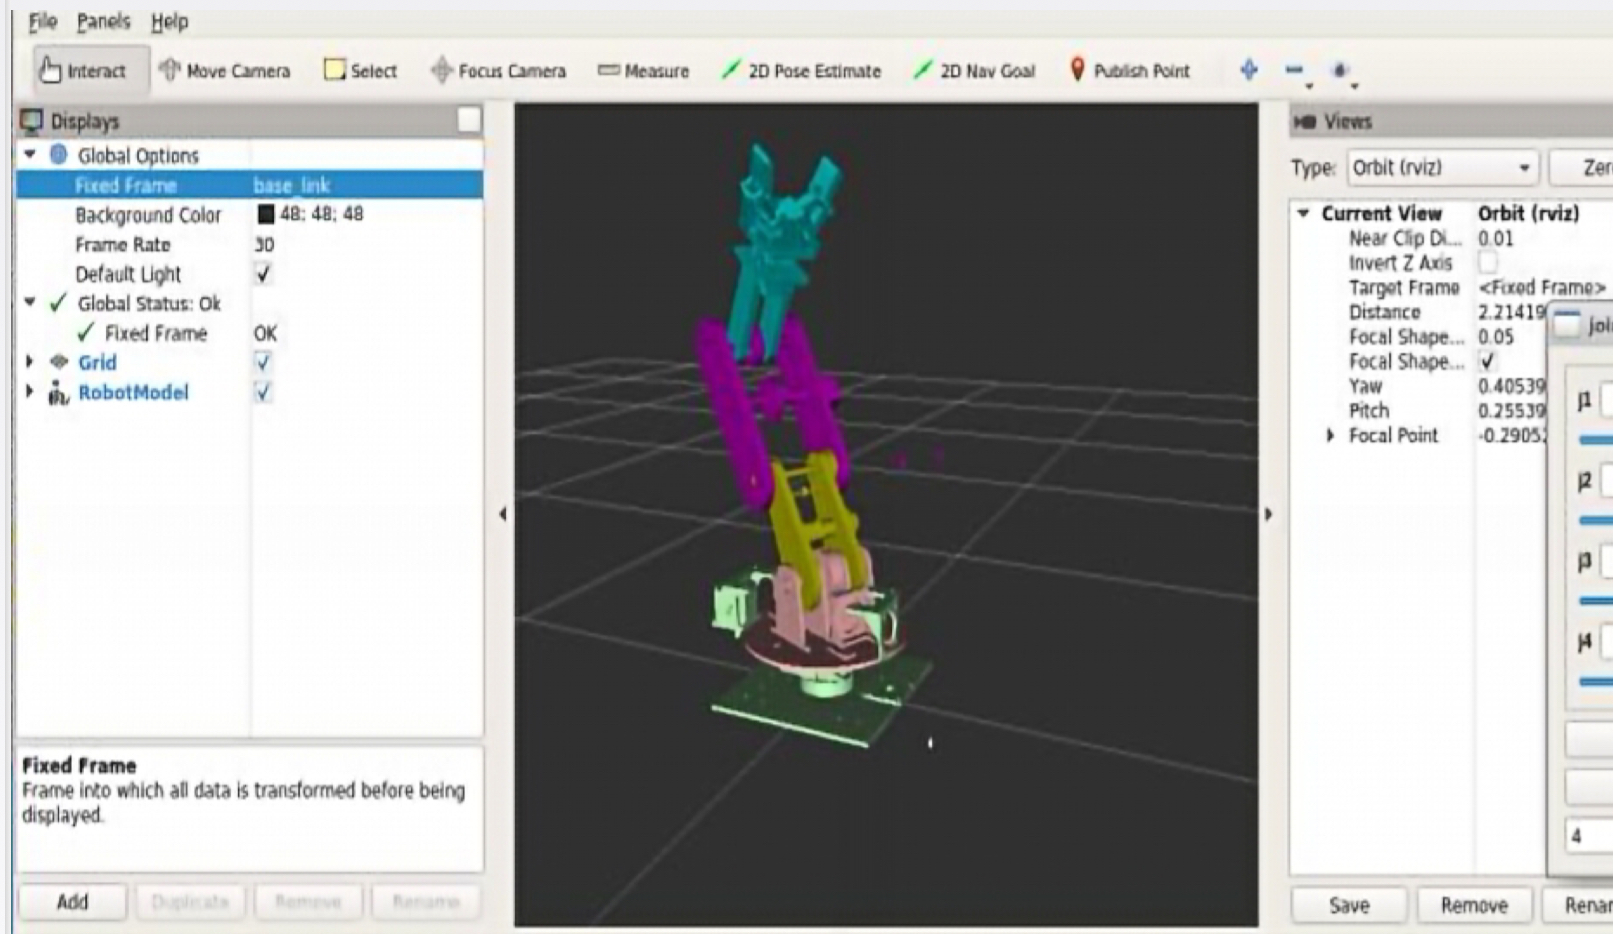
\includegraphics[width=12cm]{ros_environment_setup.jpg}
  \bicaption[ROS环境搭建]{ROS环境搭建}{ROS environment construction}
  \label{fig:ROS环境搭建}
\end{figure}